\chapter{Experimental Results}
\label{chap:todo}
During the experiments, I conducted transaction speed and scalability tests on the canister using Artillery. The main objective was to assess how quickly and efficiently the canister could process transactions. By subjecting the canister to varying levels of load, I simulated a high volume of transactions and measured the response time. The findings revealed that the canister exhibited impressive performance, maintaining a relatively fast response time even under heavy loads. This is a significant advantage as it demonstrates the canister's ability to handle a large number of transactions without compromising its efficiency, ensuring a smooth user experience.
\section{Transaction Speed}
The Internet Computer distinguishes between two types of smart contract function executions: update calls and query calls.
Update calls are requests made to modify the state of canister smart contracts. These calls initiate changes and updates within the smart contract system.
On the other hand, query calls, which constitute a significant majority (over 90\%) of the Internet Computer's traffic, are read-only requests. These calls are designed for retrieving information and do not involve any changes to the state of the smart contract. Notably, query calls are exceptionally efficient, with execution times as short as 1.5 milliseconds on the Internet Computer platform.


After conducting load testing using Artillery,As Shown in Figure \ref{fig:Canister Test} ,to evaluate the performance of the canister, we compared two sets of load testing results. The analysis of these results reveals the following observations:

For the first set of results (Query):
\begin{itemize}
    \item The maximum response time recorded was 291 milliseconds.
    \item  The 99th percentile response time, representing the response time for the vast majority of requests, was 23.8 milliseconds.
\end{itemize}

In the second set of results (Update):
\begin{itemize}
    \item The maximum response time reached 304 milliseconds.
    \item The 99th percentile response time measured at 22.9 milliseconds.
\end{itemize}

By comparing these metrics, we can see that the first set of results exhibits a slightly higher maximum response time (291 ms) compared to the second set (304 ms). However, the 99th percentile response time for the second set (22.9 ms) is lower than that of the first set (23.8 ms).

Considering the 99th percentile response time as a measure of overall performance, we can conclude that the second set of results demonstrates slightly faster performance.

It is important to note that the differences in response time between the two sets are relatively small. The choice between the sets may depend on other factors or specific requirements of the tested application or system.


\begin{figure}[H]
    \centering
    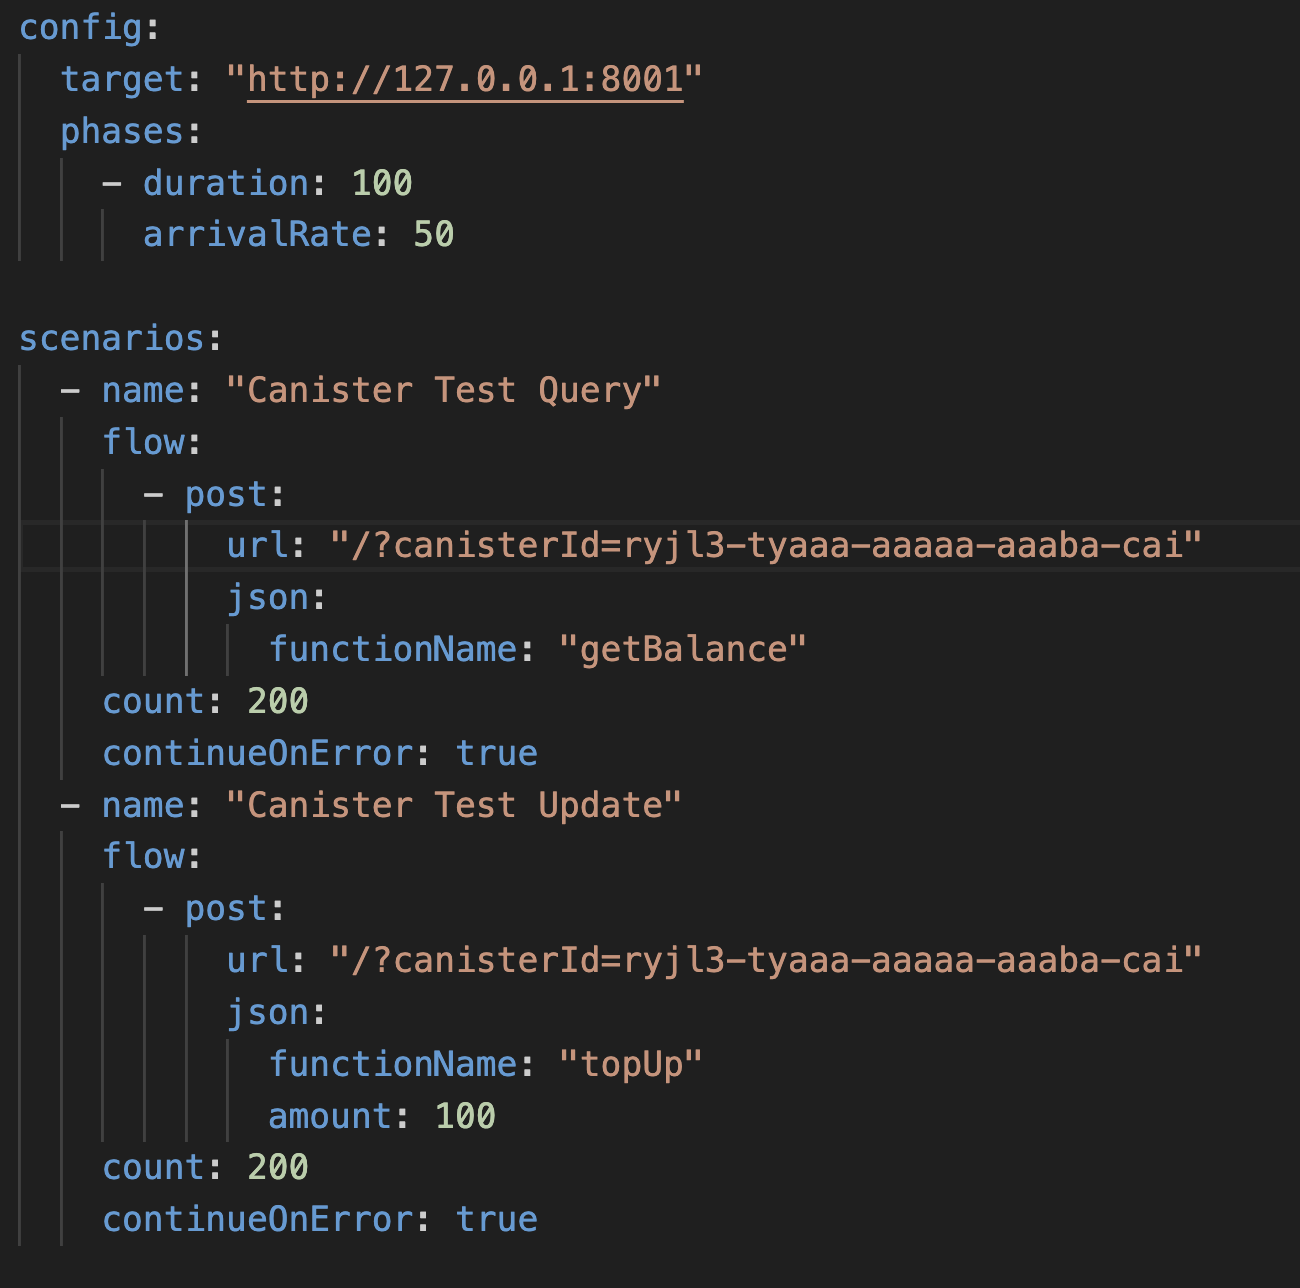
\includegraphics[width=0.8\textwidth]{test.png}
    \caption{Canister Performance Test}
    \label{fig:Canister Test}
\end{figure}


As we The following example generates 50 virtual users every second for  1.66 minutes. Both result sets have a high number of successful responses (`http.codes.200: 5000`) and completed virtual users (\`vusers.completed: 5000`). The request rate is the same (\`http.request\_rate: 50/sec`), indicating a consistent load applied in both tests.

\section{Scalability Test}

The provided test configuration ,As shown in Figure \ref{fig:Canister Scalability Test}, is designed to simulate a load on a target server running locally at "http://127.0.0.1:8001". The test consists of two scenarios: "Canister Test Query" and "Canister Test Update". During the test, 500 virtual users are created per second for a duration of 10 seconds, generating a total of 5000 requests. The "Canister Test Query" scenario involves sending a POST request to the specified URL with a JSON payload containing the function name "getBalance". Similarly, the "Canister Test Update" scenario sends a POST request with a different function name "topUp" and an amount of 100. Both scenarios are repeated 200 times, and errors encountered during the test are allowed to continue without halting the execution. Based on the test configuration, it indicates that the canister is capable of handling the load generated by 500 users per second for the given duration.

\begin{figure}[ht]
    \centering
    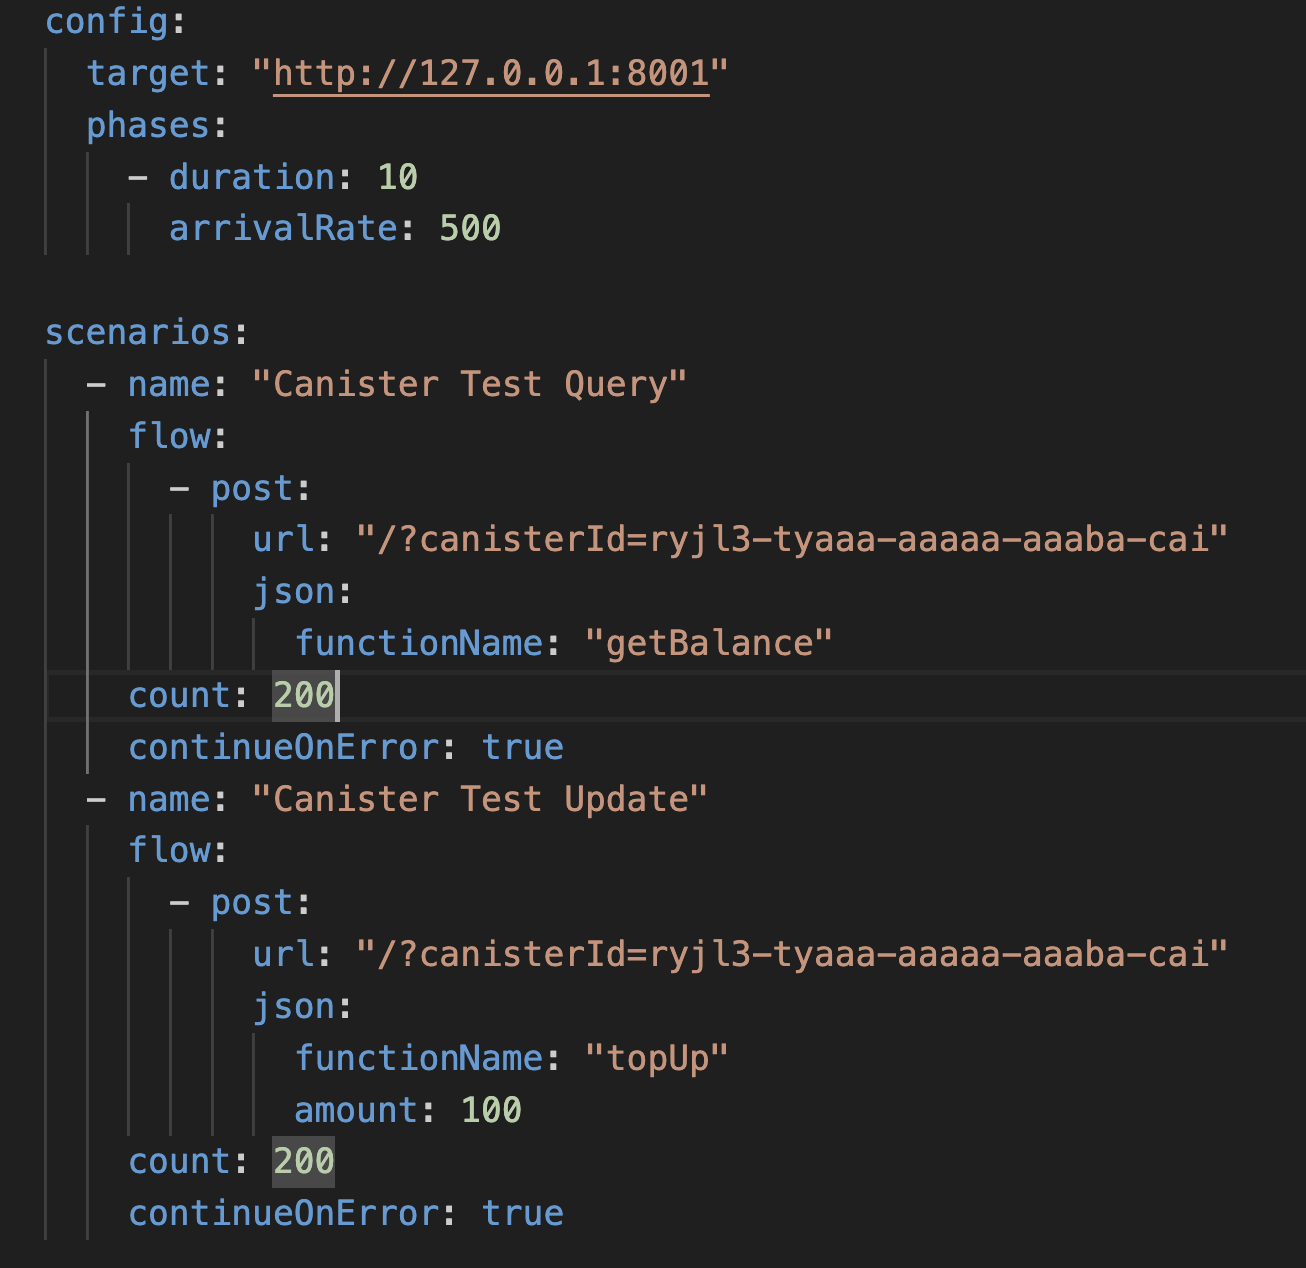
\includegraphics[width=0.8\textwidth]{Scalability.png}
    \caption{Canister Scalability Test}
    \label{fig:Canister Scalability Test}
\end{figure}

As for Table \ref{tab:performance-metrics}, the scalability testing results for the Canister application are as follows:

\begin{table}[ht]
\caption{Summary of Metrics for Scalability Test}
\centering
\begin{tabular}{ll}
\hline
\textbf{Metric} & \textbf{Value} \\
\hline
Total HTTP requests & 5000 \\
Successful HTTP responses (status code 200) & 5000 \\
Request rate & 506 requests per second \\
Minimum response time & 7 milliseconds \\
Maximum response time & 4118 milliseconds \\
Median response time & 3011.6 milliseconds \\
95th percentile response time & 3984.7 milliseconds \\
99th percentile response time & 3984.7 milliseconds \\
Total virtual users created & 5000 \\
Virtual users created for Canister Test Query & 2486 \\
Virtual users created for Canister Test Update & 2514 \\
Failed virtual users & 0\\
Minimum session length & 8 seconds \\
Maximum session length & 4210 seconds \\
Median session length & 3011.6 seconds \\
95th percentile session length & 3984.7 seconds \\
99th percentile session length & 3984.7 seconds \\
\hline
\end{tabular}
\label{tab:performance-metrics}
\end{table}

These results provide insights into the scalability of the Canister application. By analyzing the report, it is possible to assess how the system performs under load and identify any potential bottlenecks or issues related to scalability.




